\section{序論}
\label{sec:序論}
産業用ロボットは一般的に把持,搬送,組付けなどの作業をグリッパと呼ばれるエンドエフェクタで行う.グリッパは各作業用に専用設計されていることが多く,作業工程が変わるたびに交換がなされており,最適なグリッパの選定や各グリッパごとに複雑な把持計画を必要とする\cite{nishida}.近年グリッパの交換をせず様々な作業を遂行できる汎用性の高いユニバーサルグリッパの研究がなされている\cite{end}.\par
ユニバーサルグリッパにも様々な種類があり,それらは多関節グリッパ,柔軟グリッパ,内骨格型柔軟グリッパに大別される.多関節グリッパは複数の関節をもつ指を持ちそれらが対象物に倣うことで把持を行う\cite{takansetsu}.\par
多関節グリッパの代表例としてROBOTIQ社のROBOTIQ ADAPTIVE GRIPPER 3-FINGER MODELを\refig{robotiq}に示す.問題点は把持時の接触部を増やすために指の関節を増やすことが求められ機構が複雑になる点が挙げられる.\par
柔軟グリッパは把持部に柔軟膜を有し把持対象物の形状にあわせて変形する特徴がある.対象物に倣い接触面積と摩擦力を増やすことで把持を行う.柔軟グリッパの例としてジャミンググリッパがある\cite{jam}.ジャミンググリッパは柔軟膜の中に空気と粒体を有しジャミング転移現象を利用して固化し把持を行う. \par
内骨格型グリッパは内骨格と言われる固い指の表面に柔軟膜を有している.柔軟指部分が把持対象物の形状に倣いつつ内骨格による力拘束が可能である.以上の特徴から対象物の位置決め誤差や計測誤差にロバストであるとともに比較的重い物体の把持が可能である.\par
近年,組付け作業の自動化の需要が高まり汎用的な把持性能にくわえて組付け作業を想定した力覚機能が求められている.\cite{sensor}.\par
過去に開発された力覚機能をもつ柔軟指の例を紹介する.
平井らが開発したホール素子も用いた柔軟指内蔵力覚センサは柔軟指に磁石とホール素子を埋め込み,指先の変形を検知する\cite{hole}.多田らは内部に触覚受容器を持つ人間型柔軟指を開発した.金属棒と二層のシリコンゴムからなる人間の指を模した柔軟指を提案している\cite{ningen}.また,野寺らの研究によりニューラルネットワークをもちいたはめ合い技能の獲得に成功した\cite{hameai}.\par
以上の力覚機能を持つ柔軟指は産業用途における耐久性は考慮されていない.内骨格型グリッパ用に設計された耐久性と柔軟性を両立するラティス構造をもつ柔軟指が提案されている.本研究では内部にラティス構造を有し力覚センサを組み込んだ柔軟指の開発を行う.

\begin{figure}[h]
 \begin{center}
  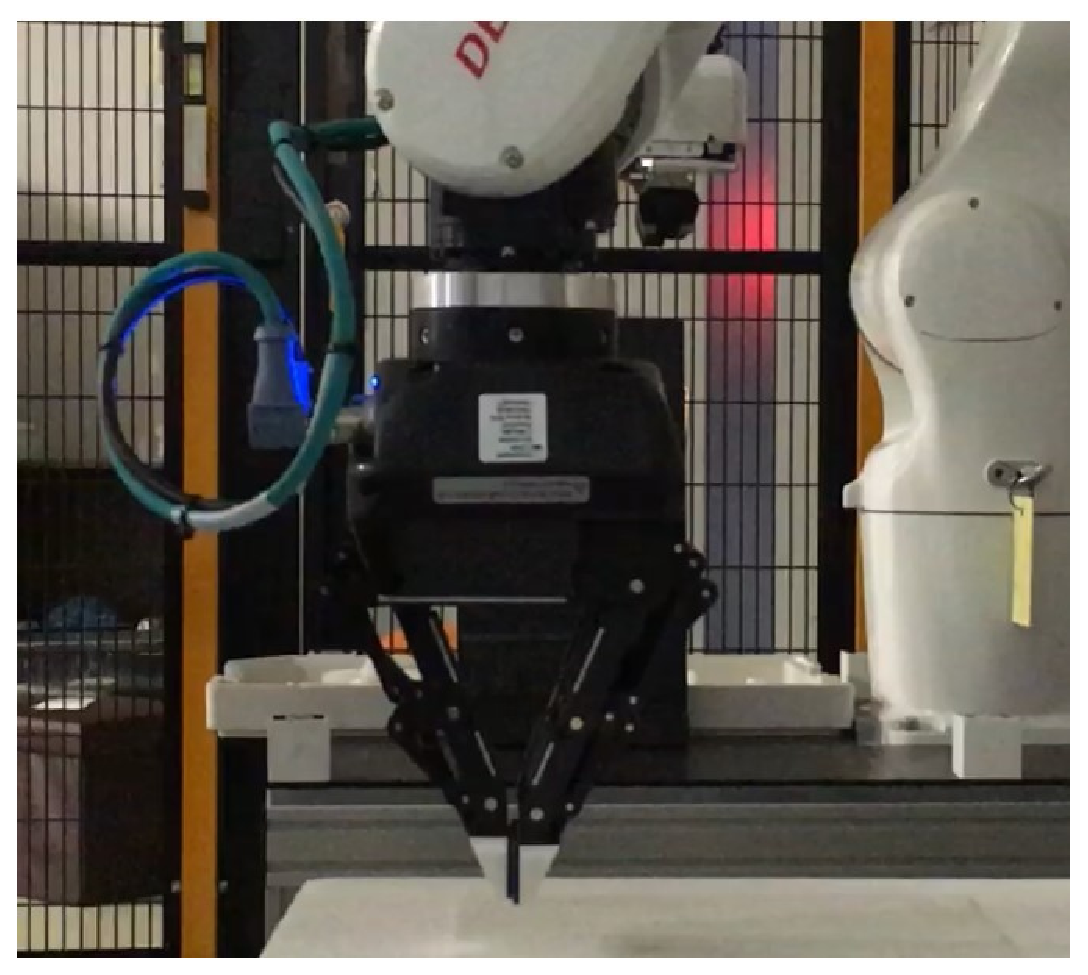
\includegraphics[scale=0.4]{../fig/eps/robotiq.eps}
 \caption{多関節グリッパ}
  \label{fig::robotiq}
 \end{center}
\end{figure}



